\section{Describe in natural language}

\tab We propose to determin some infectious diseases of pacients coming to a clinic and what is the probability of them diying. This represents a strong modality to determine the correct diagnostic ,which offers, besides the knowledge and experience of a doctor, a strong mathematical history cumulated togheter to help them.\\

\tab We will model the network starting from an example wich can be found at the following address \href{https://www.norsys.com/tutorials/netica/secA/tut_A1.html}where is presented an example taken for another diseases. The nodes will be choosen depending on our scope wich is to diagnose the patient illness wich arrives at a clinic or hospital with some affections like fever, vomiting states or muscle pain. We will determine based on this symptoms the probability of the patien to hase some specific desease. The nodes of the graph will be chosen so as to encompass the most relevant causes like if the person has been in contact with sick people, is abusing of certain substances, or has been in some regions where are registered many cases the respective desease. Besides these, will result a set of another symptoms relevant to another deseases wich can occure if the illness is not treated. \\

\tab \textbf{At the top level we have the nodes Vizita Africa with the probability of a person visiting Africa of 0.007, with 56 million tourists every year, Contact cu persoane bolnave, with a probability of 0.2, and  consum alcool/tutun, with 30pc of world population smoking and 30pc consuming alcohol daily. Those are independent nodes. A person visiting Africa can get two deadly deseases: Malaria or Yellow Fever, wich are caused by the bite of two types of mosquitoes. Every year are registered around 216 million of malaria cases, 90pc of them being in Africa, and that gives as the probability of a person getting malaria of 0.15. From the node Contact cu persoane bolnave will result flu or laryngitis wich can be caused by some type of viruses. 5 to 20pc of population is getting flu every year and 3.47 in 1000 suffers from laryngitis. Laryngitis can be also produced by alchohol and tobacco consumption. The main symptoms of malaria are coma, vomiting stats and fever. Fever is also caused by yellow fever wich is where the name comes from. Every year are registered aroung 170.000 case of yellow fever, wich gives the probability of getting yellow fever of 0.00013, raported to the population number. Flu is causing fever, pneumonia, cough or breathing problems. The main symptom of laryngitis is breathing problemes. At the bottom is de death node. A person can die of some of the deseases mentioned above.}\\

\textbf{African turism}\\
\tab One of the diseases we try to diagnosticate in this project is malaria. This represents an ifectious disease, largely spread across tropical and subtropical regions. We tried to get the number of persons, which visits annualy Africa and the number of contaminated persons with this disease. Based on statistics, Africa has a anual turism of 56 millions of people. It results that the probability of viziting Africa is =56 mil/7.5mild = 0.007.\footnote{https://qz.com/1023064/africa-is-welcoming-more-tourists-than-ever-before/}\\

\textbf{Malaria}\\
\tab International travellers could be at risk of malaria infection in 91 countries around the world, mainly in Africa, Asia and the Americas. People infected with malaria often experience fever, chills and flu-like illness at first. Left untreated, the disease can lead to severe complications and, in some cases, death. Malaria symptoms appear after a period of 7 days or longer. Fever occurring in a traveller within 3 months of possible exposure is a medical emergency that should be investigated immediately.\\

\tab Malaria is caused by the Plasmodium parasite and is transmitted by female Anopheles mosquitoes which bite between dusk and dawn. There are 5 different types of parasites that infect humans: P. falciparum, P. vivax, P. ovale, P. malariae, and P. knowlesi. Of these, P. falciparum and P. vivax are the most prevalent, and P. falciparum is the most dangerous, with the highest rates of complications and mortality. This deadly form of malaria is a serious public health concern in most countries in sub-Saharan Africa.\\

\tab WHO estimates that 216 million cases of malaria occurred worldwide in 2016 (uncertainty range: 196–263 million) and about 445 000 people died from the disease (uncertainty range: 402 000–486 000), mostly children under 5 years of age in sub-Saharan Africa. Most of the cases in 2015 were in the WHO African Region (90), followed by the WHO South-East Asia Region (7) and the WHO Eastern Mediterranean Region (2). \footnote{
 http://apps.who.int/iris/bitstream/handle/10665/252038/9789241511711\\-eng.pdf;jsessionid=85E7F9D4B20BB3EF77A00BBE23D7231D?sequence=1  (page XVII).\\
 http://www.who.int/malaria/travellers/en/\\
 -http://www.africatravelresource.com/malaria-in-africa/\\
} 

\tab According to a recent report published by the World Health Organization, malaria was responsible for the deaths of 445,000 people in 2016, with 91 per cent of fatalities occurring in Africa. \footnote{https://www.tripsavvy.com/avoid-malaria-when-traveling-in-africa-1454332}\\  

\tab Of the 216 million malaria cases reported in the same year, 90 per cent occurred in Africa. Statistics like these prove that malaria is one of the continent's most deadly diseases - and as a visitor to Africa, you are also at risk. However, with the right precautions, the chances of contracting malaria can be reduced significantly. If there are 216 million cases of malaria and 90per cent of them are in Africa, then 0.9 * 216 million = 194.4 million cases of malaria in Africa. From this probability we can get the probability of getting malaria if you go in Africa:\\
		\tab \tab \textbf{=> p(M|A) = 194.4 mil / 1.26 bil. = 0.15,} \\
1.26 bil. being the population of Africa.\\

\tab According to statistics recorded over several decades, the likelihood of a person being infected with malaria if he did not visit Africa is 2 per cent.\\

\begin{center}
  	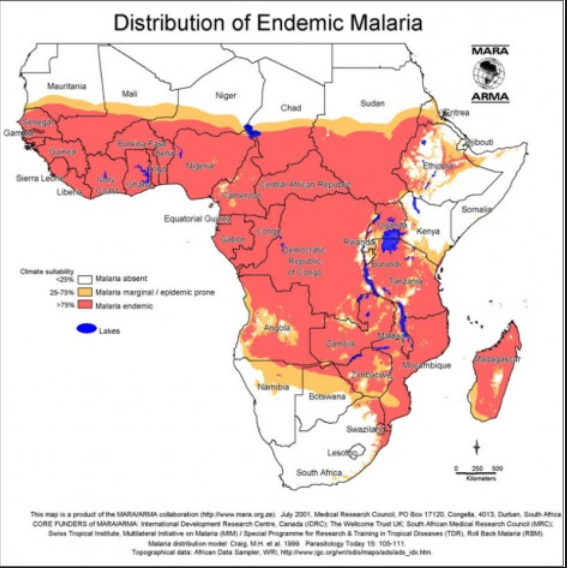
\includegraphics[scale=0.8]{malaria.png}
\end{center}

\textbf{Yellow Fever}\\
\tab Yellow fever is caused by the yellow fever virus, which is carried by mosquitoes. It is endemic in 33 countries in Africa and 11 countries in South America. The yellow fever virus can be transmitted by mosquitoes which feed on infected animals in forests, then pass the infection when the same mosquitoes feed on humans travelling through the forest. The greatest risk of an epidemic occurs when infected humans return to urban areas and are fed on by the domestic vector mosquito Aedus aegypti, which then transmits the virus to other humans.\\

\tab Symptoms of yellow fever include fever, headache, jaundice, muscle pain, nausea, vomiting and fatigue. 
 A small proportion of patients who contract the virus develop severe symptoms and approximately half of those die within 7 to 10 days. \\

\tab The virus is endemic in tropical areas of Africa and Central and South America. Large epidemics of yellow fever occur when infected people introduce the virus into heavily populated areas with high mosquito density and where most people have little or no immunity, due to lack of vaccination. In these conditions, infected mosquitoes of the Aedes aegypti specie transmit the virus from person to person. \\

\tab Yellow fever is prevented by an extremely effective vaccine, which is safe and affordable. A single dose of yellow fever vaccine is sufficient to confer sustained immunity and life-long protection against yellow fever disease and a booster dose of the vaccine is not needed. The vaccine provides effective immunity within 30 days for 99 per cent of persons vaccinated. \footnote{ http://www.who.int/mediacentre/factsheets/fs100/en/}\\

\tab Forty seven countries in Africa (34) and Central and South America (13) are either endemic for, or have regions that are endemic for, yellow fever. A modelling study based on African data sources estimated the burden of yellow fever during 2013 was 84 000–170 000 severe cases and 29 000–60 000 deaths.\\

\tab There are 170.000 cases of yellow fever anually in Africa, and to get the probability of yellow fever occuring, we divide the number of registered cases to the Africa’s population:\\

	\tab \tab \textbf{p(FG/A) = 170.000/1.26 mild = 0.00013}\\

\tab The probability to get yellow fever if you not vizit Africa is very small : 0.00001.\\

\begin{center}
  	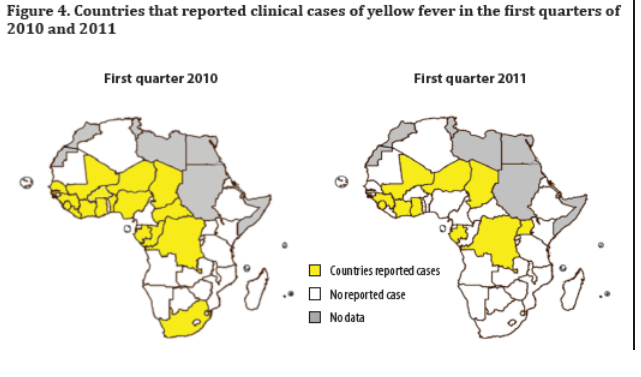
\includegraphics[scale=0.8]{yellowfever.png}
\end{center}


\textbf{Contact with sick people}\\
\tab We assume that the probability to get contact with sick people is 20 per cent during daily activities.\\

\textbf{Alcohol and smoking}\\
\tab
•	About a third of the male adult global population smokes.\\
•	Smoking related-diseases kill one in 10 adults globally, or cause four million deaths. By 2030, if current trends continue, smoking will kill one in six people.\\
•	Every eight seconds, someone dies from tobacco use.\\
•	Smoking is on the rise in the developing world but falling in developed nations. Among Americans, smoking rates shrunk by nearly half in three decades (from the mid-1960s to mid-1990s), falling to 23 pc of adults by 1997. In the developing world, tobacco consumption is rising by 3.4pc per year.\\
•	About 15 billion cigarettes are sold daily - or 10 million every minute.\\
•	About 12 times more British people have died from smoking than from World War II.\\
•	Cigarettes cause more than one in five American deaths.\\
•	Among WHO Regions, the Western Pacific Region* - which covers East Asia and the Pacific - has the highest smoking rate, with nearly two-thirds of men smoking.\\
•	About one in three cigarettes are consumed in the Western Pacific Region.\\
•	The tobacco market is controlled by just a few corporations - namely American, British and Japanese multinational conglomerates.\\
\begingroup\makeatletter\def\@currenvir{verbatim}
\verbatim
The proportion of the population who consumed alcohol daily declined between
 2007 (8.1%) and 2010 (7.2%) 1. 
•  A higher proportion of 12-17 year olds abstained from alcohol (61.6%) than 
had consumed it in the last 12 months (38.4%) 1. 
•  The proportion of 12-15 year olds and 16-17 year olds abstaining from alcohol
 increased in 2010 (from 69.9% in 2007 to 77.2% in 2010 and from 24.4% to 31.6%, respectively) 1. 
•  In 2010, 1 in 5 people aged 14 years or older consumed alcohol at a level that 
put them at risk of harm from alcohol-related disease or injury over their lifetime, and this remained 
stable between 2007 (20.3%) and 2010 (20.1%). However, the number of people drinking in risky 
quantities increased from 3.5 million in 2007 to 3.7 million in 2010 1. 
•  About 2 in 5 (39.7%) people aged 14 years or older drank, at least once in
 the last 12 months, in a pattern that placed them at risk of an alcohol-related injury from a single 
drinking occasion; but there was a modest by statistically significant decline in risky drinking over the previous
 12 months from 2007 (41.5%) 1. 
•  Males were far more likely than females to consume alcohol in risky quantities, 
and those aged between 18-29 years were more likely than any other age group to consume 
alcohol in quantities that placed them at risk of an alcohol-related injury, and of alcohol-related 
harm over their lifetime 1. 
•  The proportion of pregnant women abstaining during pregnancy increased in 2010 (from 40
% in 2007 to 52% in 2010).
\end{verbatim}


\textbf{According to world-wide statistics, about 7pc of the population regularly consume alcoholic and 30 pc of them tobacco.}\\

\textbf{Coma}\\
\tab The outcome of a patient can be associated with their best response in the first twenty-four hours after injury. Using the Glasgow Coma Scale (3 to 15, with 3 being a person in a coma with the lowest possible score, and 15 being a normal appearing person) research shows that if the best scale is 3 to 4 after twenty four hours, 87pc of those individuals will either die or remain in a vegetative state and only 7pc  will had a moderate disability or good recovery. In patients with a scale from 5 to 7, 53pc  will die or remain in a vegetative state, while 34pc  will have a moderate disability and/or good recovery. In patients with a Glasgow Coma Scale of 8 to 10, 27pc  will die or remain in a coma, while 68pc  will have a moderate disability and/or good recovery. In patients who have a scale from 11 to 15, only 7pc  will be expected to die or remain in a coma, while 87pc  would expect to have at least a moderate disability and/or good recovery (remembering again that this is not an exact science).\footnote{http://www.braininjury.com/coma.shtml}\\

\textbf{Influenza}
\tab Influenza is an acute viral infection that primarily attacks the upper respiratory tract, including the nose, throat, bronchi and, less frequently, the lungs. The disease occurs worldwide and spreads very quickly in populations, especially in crowded circumstances. In the northern hemisphere, annual influenza epidemics occur during autumn and winter affecting approximately 5-20pc of the population.\\

\tab \textbf{5 to 20pc} -- Percentage of the U.S. population that will get the flu, on average, each year.\\
\tab \textbf{200,000} -- Average number of Americans hospitalized each year because of problems with the illness\\
\tab 3,000 to 49,000 -- Number of people who die each year from flu-related causes in the U.S.\\
\tab 10 billion+ -- Average costs of hospitalizations and outpatient doctor visits related to the flu.\\
\tab 1 to 4 days -- Typical time it takes for symptoms to show up once you've caught the virus. Adults can be contagious from the day before symptoms begin through 5 to 10 days after the illness starts.\footnote{http://www.euro.who.int/en/health-topics/communicable-diseases/influenza/data-and-statistics\\
https://www.webmd.com/cold-and-flu/flu-statistics\\
}\\

\tab According to statistics, inluenza affects 12pc of people who make contact with other sick people. In the other cases, influenza affects approximately 4pc  of the people.\\
\tab \tab p(G|CPB) = 12pc , P(G|-CPB) = 4pc , where G represents influenza and CPB represents contact with sick people.\\


\textbf{Laryngitis}

METHODS: 
We retrospectively identified patients with a diagnosis of CL who were seen among a primary care cohort at an urban academic medical center from 2009 to 2010. The incidence of CL was calculated. Symptoms, first-visit treatment, smoking, and demographics were recorded.
RESULTS: 
Of a population of 40,317 people, 280 received a new diagnosis of CL over a 2-year period, representing a yearly incidence of 3.47 cases per 1,000 people. The subjects consisted of 160 women and 120 men. Race was recorded as black (126), Hispanic (47), white (68), or other (39). The mean age was 52.9 years (range, 20 to 90 years). The initial therapies included proton pump inhibitors (79pc, voice therapy (17pc), nasal steroid (13pc), antihistamine (4pc), amitriptyline (4pc), other (17pc), and none (11pc). The most common symptoms were dysphonia (53pc), pain/soreness (45pc), globus sensation (40pc), cough (33pc), excessive throat clearing (28pc), and dysphagia (32pc). An otolaryngologist saw 93pc of the cases.\\
CONCLUSIONS: 
The yearly CL incidence was 3.47 per 1,000 people. Up to 21pc of the population may develop CL in their lifetime. Most of the patients in this cohort were referred to otolaryngologists, and the majority were treated with proton pump inhibitors. Dysphonia, globus sensation, and pain were the most common symptoms. Population surveys could be used to define undiagnosed disease and the overall prevalence of CL.\\

\section {Querries and diagram}

\tab The diagram of all the nodes and combinations of those is here.\\

\begin{center}
  	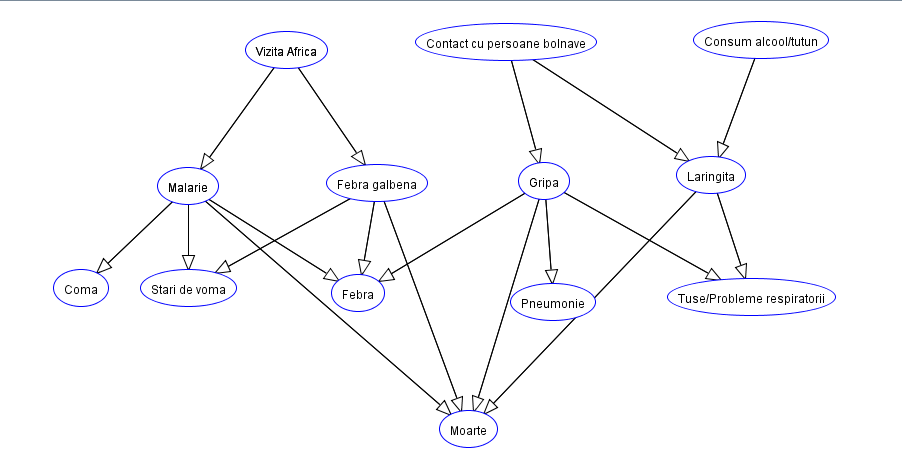
\includegraphics[scale=0.5]{diagrama}
\end{center}

\tab The result tab with all the probability tables is shown here + a querry on the result of ours from which we can conclude that there is a change of \textbf{0.0009} to be killed by malaria, or yellow fever or flu..etc. The best contributant to this is flu , because it affects almost all the people , while malaria and yellow fever are scarced and dependes on lot of factors to get them.\\

\begin{center}
  	\includegraphics[scale=0.8]{diagramwithProb}
\end{center}
